\section{STRIDE Modeling}
\subsection{Overview}
STRIDE is one of the most mature threat analysis modeling methods. Microsoft has adopted this method since 2002, where STRIDE stands for, Spoofing, Tampering, Repudiation, Information disclosure, Denial of Service, and Elevation of privilege \citep[p.~1]{shevchenko2018threat}. Its simplicity and ability to find threats using dataflow diagrams made it a promising candidate for this report.\newline\newline
Figures \ref{fig:dfd_staff} and \ref{fig:dfd_user} depict a Level 0 dataflow diagram concerning different actors and how the system acts between trusted boundaries. Additionally, from the DFD, we can identify events and boundaries of the ASMIS system that would provide a concrete platform to perform STRIDE modeling \citep[p.~1]{shevchenko2018threat}.

\begin{figure}[h!]
\centering
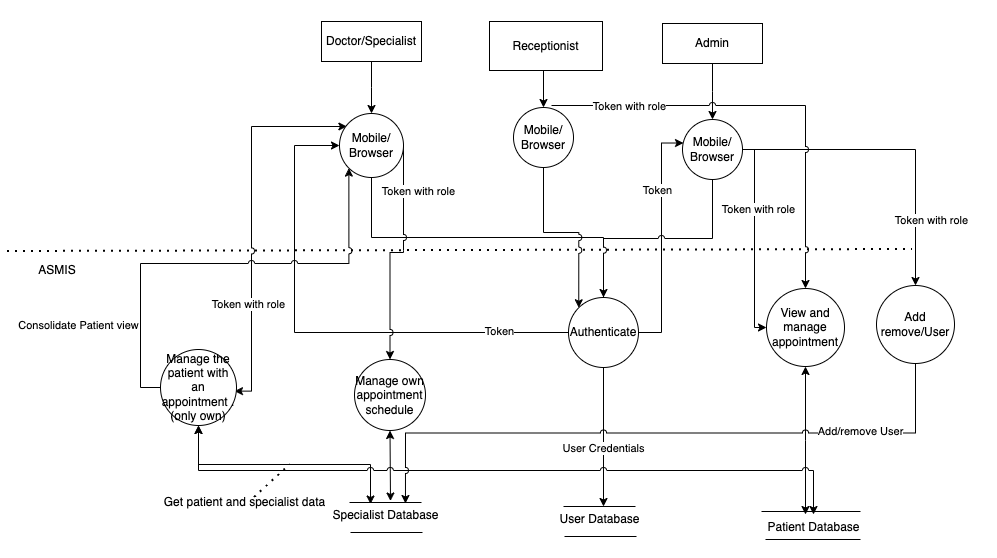
\includegraphics[width=16cm, height=11cm]{pics/dfd_staff.png}
\caption{DFD level 0 Staff for ASMIS}\label{fig:dfd_staff}
\end{figure}

\begin{figure}[h!]
\centering
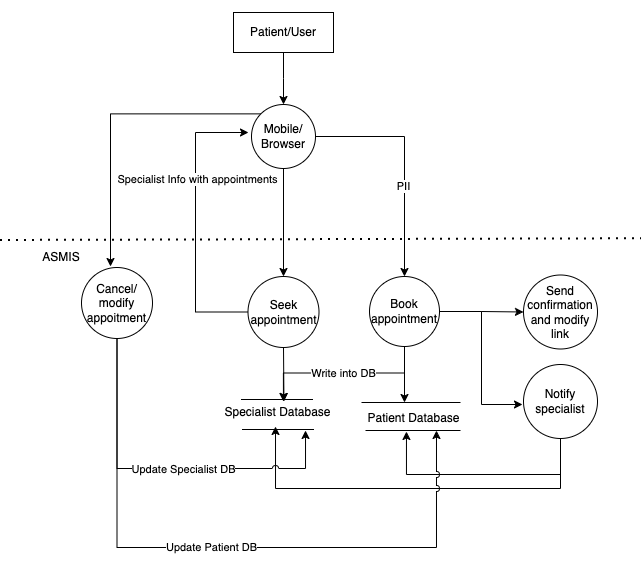
\includegraphics[width=12cm, height=11cm]{pics/dfd_user.png}
\caption{DFD level 0 User for ASMIS}\label{fig:dfd_user}
\end{figure}


\subsection{Spoofing}
\begingroup
\centering
\setlength{\tabcolsep}{6.5pt} % Default value: 6pt
\renewcommand{\arraystretch}{1.8} % Default value: 1
\begin{longtable}{ |p{7cm}| p{8cm} |}
\caption{Spoofing Mitigations and threats}
    \label{table:spoofing}
\hline
\textbf{Threats} & \textbf{Mitigations}\\
\hline
Staff account is compromised & Having strict MFA rules for the staff.\newline 
Using only app-based or hardware key-based MFA solutions. \\
\hline
DNS spoofing to redirect users to a fake site & Use DNSSec to prevent cache poisoning. \\
\hline
Ip spoofing & Network monitoring, and a firewall should be utilized.\\
\hline
An attacker can pose as an unauthenticated user to make appointments unavailable & Use robust authentication techniques, like MFA (SMS), to verify users before confirming the appointments.\\
\hline
Replay attacks & Use only one-time usable refresh tokens and blacklist all tokens if the refresh token is used more than once.\\
\hline
Man-in-the-middle-attack & Use encrypted protocols, i.e., HTTPS/SSL, TLS, everywhere to communicate.\newline
Keeping the validity of the access tokens short-lived. \\
\hline
\end{longtable}
\endgroup

\subsection{Tampering}

\begingroup
\centering
\setlength{\tabcolsep}{6.5pt} % Default value: 6pt
\renewcommand{\arraystretch}{1.8} % Default value: 1
\begin{longtable}{ |p{7cm}| p{8cm} |}
\caption{Tampering Mitigations and threats}
    \label{table:tamp}
\hline
\textbf{Threats} & \textbf{Mitigations} \\
\hline
Tampering roles in a token of an authorized user & Digital signatures using a safely stored private key on the tokens should be carried out.\\
\hline
Injection of malicious code in application code. & Using checksums to test the recognized codes.\\
\hline
Cross-Site Request Forgery & Using CSRF token to verify the request.\\
\hline
Modify a patient's appointments without authority & Sending OTP to patient's verified phone before being able to modify appointments.\\
\hline
\end{longtable}
\endgroup



\subsection{Information Disclousre}

\begingroup
\centering
\setlength{\tabcolsep}{6.5pt} % Default value: 6pt
\renewcommand{\arraystretch}{1.8} % Default value: 1
\begin{longtable}{ |p{7cm}| p{8cm} |}
\caption{Information Disclosure Mitigations and threats}
    \label{table:info_dis}
\hline
\textbf{Threats} & \textbf{Mitigations}\\
\hline
SQL injection to get data from the database & Use proven frameworks which has safe functions for databases.\\
\hline
Sensible keys are retrieved from the application. & Store secret keys in a Keystore separate from the application.\\
\hline
Weak database password &  Regularly rotate keys, i.e., 90 days. \newline
Use IAM short-lived roles instead of long-lived keys to access databases. \\
\hline
Get valuable information from network analysis & Use a firewall or redirect malicious requests to a honeypot \citep{manageengine}.\\
\hline
Sensible data is exposed & Hash sensible passwords using strong algorithms like argon2 and bcrypt. \citep{owasp_secure_encrypt}\\
\hline
\end{longtable}
\endgroup

\subsection{Redupation}
\begingroup
\centering
\setlength{\tabcolsep}{6.5pt} % Default value: 6pt
\renewcommand{\arraystretch}{1.8} % Default value: 1
\begin{longtable}{ |p{7cm}| p{8cm} |}
\caption{Redupation Mitigations and threats}
    \label{table:redupation}
\hline
\textbf{Threats} & \textbf{Mitigations}\\
\hline
Claims to be some other user/staff & Audit the changes by the users.\\
\hline
A user claims to have yet to set up or cancel an appointment. & Use timestamps for services and APIs used.\\
\hline
\end{longtable}
\endgroup


\subsection{Denial of Service}
\begingroup
\centering
\setlength{\tabcolsep}{6.5pt} % Default value: 6pt
\renewcommand{\arraystretch}{1.8} % Default value: 1
\begin{longtable}{ |p{7cm}| p{8cm} |}
\caption{DoS Mitigations and threats}
    \label{table:dos}
\hline
\textbf{Threats} & \textbf{Mitigations} \\
\hline
Attempt too many logins for staff & Only allow patients to book appointments with verifying, i.e., Use of phone numbers verification. \newline
Restrict the number of appointments a patient can make within a certain period.\\
\hline
Use bots to carry out Syn flood attacks on the application & Use a CDN to offload the servers.\newline 
Use a WAF or DDoS protection tool like Cloudflare in front of the services.\newline
Monitor/alerting for network logs.\newline
Use ML tools that scan and block blacklisted IPs.
\\
\hline
\end{longtable}
\endgroup


\subsection{Elevation of Privilege}

\begingroup
\centering
\setlength{\tabcolsep}{6.5pt} % Default value: 6pt
\renewcommand{\arraystretch}{1.8} % Default value: 1
\begin{longtable}{ |p{7cm}| p{8cm} |}
\caption{Elevation of Privileges Mitigations and threats}
    \label{table:eop}
\hline
\textbf{Threats} & \textbf{Mitigations} \\
\hline
Admin Privileges to all the staff & Use least privilege principal and give permissions needed only.
\\
\hline
A super user for the application, which could access all the resources. & Use least privilege principle.\\
\hline
Unauthorized roles are added to a user & Use rigorous MFA methods to verify a change of roles.
\hline
\end{longtable}
\endgroup


